\documentclass[a4paper]{jsarticle}

\usepackage[dvipdfmx, hiresbb]{graphicx}
\usepackage{macros}

\newcommand{\Cov}{\operatorname{Cov}}

\begin{document}
\title{ゼミノート \#2 \\ Sites and Sheaves}
\author{七条彰紀}
\maketitle

\section{Motivation.}
scheme, stack等には以下のような包含関係がある.
\[\xymatrix{
    {} & \text{Algebraic Stack} \ar@{^{(}->}[r]& \text{Stack} \ar@{^{(}->}[r]& \text{Presheaf of Grupoids} \\
    \text{Scheme} \ar@{^{(}->}[r]\ar@{^{(}->}[ru]& \text{Algebraic Space} \ar@{^{(}->}[r]\ar@{^{(}->}[u]&
        \text{Space} \ar@{^{(}->}[r]\ar@{^{(}->}[u]& \text{Presheaf of Sets} \ar@{^{(}->}[u]
}\]
最終的にセミナーを通じて我々が定義したいのはalgebraic stackであるが,
今回はそれよりも定義が簡素な``space"を定義する.
先にspaceの定義文を示そう.

\begin{Def}[Space, \cite{GomezAS} p.26]
    $S$ :: schemeとする.
    Space over $S$ (or $S$-space)とは,
    big etale site over $S$上にある,集合のsheafである.
\end{Def}
ここに現れる``big etale site"と``big etale site上のsheaf"を以下で定義する.
さらにsheafの射について幾つか定義をすれば,
algebraic spaceまで定義できる.

定義だけではspaceのlocalは性質を調べる手段がないため,
次回は「高次版のsheafの貼り合わせ」と呼べる``Descent theory"を学ぶ.

\section{Definitions : Sites.}
以下で導入するGrothendieck topologyは,
「Sheafを定義するのに必要な位相空間の定義を抽出し,圏論的に一般化したもの」である.
$X$ :: toplological spaceとし,sheaf on $X$の定義を見なおしてみよう.
すると,sheaf on  $X$は次に挙げるもののみを用いて定義されていると分かる.
\begin{enumerate}
    \item $X$の開部分集合と包含写像が成す圏.
    \item 開部分集合$U \subseteq X$のopen covering.
    \item 同じく$U$のopen covering :: $\{U_i\}_i$が与えられたときの族$\{ U_i \cap U_j \}_{i,j}$
\end{enumerate}

\begin{Def}[Grothendieck Topology]
    $\cat{C}$ :: cateogoryについて,
    $\cat{C}$上のGrohendieck topologyは
    任意の$X \in \cat{C}$に
    $\cat{C}$の射の集まり(collection)$\{X_i \to X\}_{i \in I}$を対応させる$\Cov$で構成される.
    さらに,$\Cov$は以下を満たすように要請される.
    \begin{enumerate}[label=(\alph*)]
        \item
            $X' \to X$ :: isoならば$\{X' \to X\} \in \Cov(X)$.
        \item
            $\{U_i \to U\} \in \Cov(U), V \to U \in \cat{C}$について,
            $\{U_i \times_U V \to V\} \in \Cov(V)$.
        \item
            $\{U_i \to U\}_i \in \Cov(U)$をとり,
            さらに各$i$について$\{V_{i,j} \to U_i\}_j \in \Cov(U_i)$をとる. \mbox{}\\
            この時,合成も$\Cov$に入っている : $\{V_{i,j} \to U_i \to U\}_{i,j} \in \Cov(U)$.
    \end{enumerate}
\end{Def}

\begin{Remark}\label{rem:grotop_stablecond}
    $\Cov$の条件のうち,
    (b), (c)はそれぞれstable under base change, stable under compositionに対応する.
\end{Remark}

\begin{Def}[Site]
    圏$\cat{C}$と$\cat{C}$上のGrothendieck topology :: $\Cov$の組をsiteと呼ぶ.
\end{Def}

\section{Examples : Sites.}
\begin{Example}[Classical topology.]
    
\end{Example}

以下で実際に用いるのは,
$\cat{C}$がslice category :: $\Sch/X \ (X \in \Sch)$の部分圏であるようなsiteである.
$X \in \Sch$に対して,
このようなsiteは圏と$\Cov$からなるから,
以下の図の(a) $U$, (b)$U \to X$, (c) $U_i \to U$がどのようなものであるか定めれば定義できる.
\begin{center}
     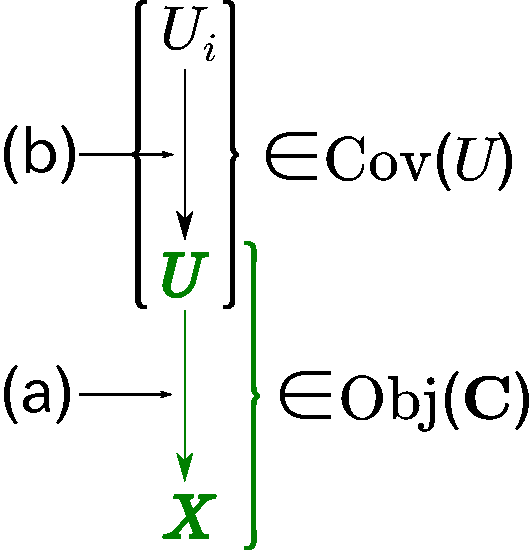
\includegraphics[width=5cm]{./images/site.pdf}
\end{center}
すなわち,以下の未完成な定義文をテンプレートとする,一連の定義文の群がある.
\begin{Def}[$***$ site]
    $X$ :: schemeについて,
    圏$\cat{C}$を以下で定める.
    \begin{description}
        \item[対象] (a)であるscheme :: $U$から$X$への,(b)である射$U \to X$.
        \item[射]   二つの対象の間の射$[U \to X] \to [U' \to X]$は,$X$-morphism :: $U \to U'$.
    \end{description}
    $[U \to X] \in \cat{C}$に対して,$\Cov(U)$を以下のような集まりとする:
    (c)を満たす射の集まり$\{U_i \to U\}_i$であって
    \[ \bigsqcup_i U_i \to U \]
    がsurjectiveであるものからなる集まりが$\Cov(U)$.

    以上の$\cat{C}$と$\Cov$からなるsiteを $***$ siteと呼ぶ.
\end{Def}

注意(\ref{rem:grotop_stablecond})で触れたとおり,
性質(c)がstable under base change \& compositionであれば,
以上のテンプレートはsiteの定義文と成る.

\begin{Def}
%% ***とa,b,cの表にする.    
\end{Def}

\section{Definitions : Sheaves.}

\section{Examples : Sheaves.}

\section{Propositions : Sheaves.}

\section{Definitions : Morphism of Shaves.}

\section{Examples : Morphism of Shaves.}


\bibliographystyle{jplain}
\bibliography{reference}
\end{document}
